\documentclass{rapportECL}
\usepackage{lipsum}
\usepackage{biblatex} %Imports biblatex package
\addbibresource{bibliotheque.bib}

\title{Rapport ECL - Template} %Titre du fichier

\begin{document}

%----------- Informations du rapport ---------

\titre{Un Langage "Pur" pour Web Assembly} %Titre du fichier .pdf
\UE{PSTL} %Nom de la UE

\enseignant{Frédéric \textsc{Peschanski}} %Nom de l'enseignant

\eleves{Lucas \textssc{Fumard} \\
	Lauryn \textsc{Pierre} \\
	Saïd Mohammad \textsc{ZUHAIR} } %Nom des élèves

%----------- Initialisation -------------------

\fairemarges %Afficher les marges
\fairepagedegarde %Créer la page de garde
\tabledematieres %Créer la table de matières

%------------ Corps du rapport ----------------
\section{Introduction}
Le but de notre projet est de concevoir un langage 100 $\%$ fonctionnel et “pur” pour WebAssembly en 
se basant sur cet article\cite{ullrich_counting_2020}(fourni). L'article défini un langage fonctionnel dont la gestion de la mémoire se fait par 
un mécanisme de comptage de références.
WebAssembly\cite{noauthor_webassembly_nodate} ou Wasm définit un format de code binaire portable
et un langage de type assembleur\cite{noauthor_webassembly_2023}. Tous les principaux navigateurs peuvent exécuter des programmes WebAssembly. 
Des langages comme C, C++, Rust, Go et bien d'autres peuvent être compilés en WebAssembly.
Plusieurs compilateurs ont été développés pour WebAssembly\cite{noauthor_wabt_2023,noauthor_wasm3_2023,noauthor_wasmer_nodate,noauthor_wasmtime_nodate}. 

\section{WebAsssembly}
WebAssembly\cite{noauthor_webassembly_nodate} est un langage bytecode pris en charge par les principaux navigateurs
Web, conçu principalement pour être une cible de compilation efficace pour les langages de bas niveau tels que C/C++ et Rust.
Les applications de WebAssembly ne se limite pas qu'au Web,il y a également un intérêt pour l'Internet des Objets, les serveurs.
WebAssembly a un format texte(.wat) et un format binaire(.wasm). 
Dans le cas de notre projet on utilise wabt\cite{noauthor_wabt_2023} pour compiler et on exécute le compilé à l’aide de Node.js\cite{noauthor_nodejs_nodate}

\section{Cahier des charges}
Les tâches que nous avons identifié sont les suivantes :

- Analyser le fonctionnement de WASM

- Programmer un parseur qui puisse lire le langage pur tel que défini dans l'article\cite{ullrich_counting_2020}

- Programmer un interpréteur en Rust du langage selon les sémantiques du langage pur

- Définir quelques tests unitaires couvrant les sémantiques définies dans l'article

- Ajouter la gestion des instructions \verb|inc|, \verb|dec|, \verb|reset|, \verb|reuse|

- Programmer un compilateur du langage agrandi vers WASM

\section{Tâches Réalisées}

\subsection{Lecture de l'article}
Le langage fonctionnel décrit dans l'article\cite{ullrich_counting_2020} alloue ses constructeurs dans la pile et manipule des 
adresses vers ces emplacements mémoire alloués. Il est donc primordial d'avoir un système d'allocation et réutilisation de 
mémoire performant afin d'éviter les fuites mémoires et un temps d'exécution faible.

Le système de la gestion de la mémoire par comptage de référence est bien plus vieux que des systèmes par garbage collector, 
mais aussi plus efficaces\cite{ullrich_counting_2020}. Cependant, la gestion de mémoire comptage de références ne fonctionne que si 
il n'est pas possible de créer de cycle de référence. 
C'est pourquoi les garbage collector sont plus utilisés de nos jours.

Les auteurs de l'article\cite{ullrich_counting_2020} ont créé un langage fonctionnel dans lequel les cycles de références 
sont impossibles afin d'implémenter un système de gestion de mémoire par comptage de référence et d'obtenir un langage fonctionnel 
dont l'exécution est optimisée. C'est ce langage que nous allons implémenter.

\subsection{Parser/reader}
Concernant la grammaire du langage, nous avons décidé de garder celle définie à la section 3 de l'article que voici.
\begin{center}
	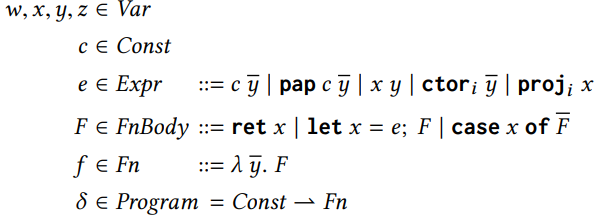
\includegraphics[scale=0.65]{logos/grammaire.png}	
\end{center}
Notre reader utilise la bibliothèque Chumsky\cite{zesterer_chumsky_nodate}, ainsi nous ne pouvons pas stoquer les noms définis 
variable ce qui nous empêche de distinguer directement les constantes des variables.

\subsection{Interpréteur}

Afin d'implémenter un interpréteur du langage décrit, il nous a d'abord fallu implémenter les structures permettant d'accéder à la mémoire.

\begin{center}
	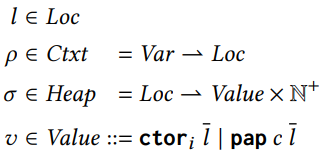
\includegraphics[scale=0.65]{logos/figure_strutures_interpreteur.png}	
\end{center}

\verb|Loc| est l'adresse de la case mémoire allouée pour la valeur dans la pile. C'est la valeur de retour de toutes les sémantiques 
du langage, tel que définies dans la figure 1 de l'article\cite{ullrich_counting_2020}.
Contrairement à l'article, nous avons choisi de ne pas retourner une nouvelle pile à chaque fois, mais de garder une même pile que 
l'on modifie par effet de bord. 

Nous avons testé cet interpréteur en créant plusieurs tests unitaires sur les sémantiques mais aussi quelques programmes simples, 
tel que le calcul de fibonacci, ou le programme \verb|swap| défini à la page 5 de l'article\cite{ullrich_counting_2020}.

\section{Tâches Restantes}

Il nous faut choisir un schéma de mémoire pour les objets dans la mémoire.
Il nous faut implémenter \verb|inc|, \verb|dec|, \verb|reset|, \verb|reuse|.
Il nous faut faire le compilateur en WASM

WASM n'a qu'un seul type de variable : les nombres (entiers ou flottant, 32 bit ou 64 bit). 
Ainsi, il faut que l'on interprète différement ces nombres selon le contexte dans lequel on les prend. 
Dans la mémoire, nos constructeurs et applications partielles seront stoqués sous la forme \verb|<type> <nombre de références> <arguments>|. 
Par exemple, une application partielle est sous la forme \verb|6 1 7 2 12 13| où 6 est le type "application partielle", 
1 est le nombre de références à cette application partielle, 
7 est l'identifiant de la fonction à appeler (dans l'interpréteur, on utilise des \verb|string|), 
2 est le nombre d'arguments fixés et 12 et 13 sont les arguments fixés.

Dû à la difficulté d'une telle tâche, nous laissons l'implémentation des applications partielles pour plus tard.

\printbibliography
\end{document}